\documentclass[aspectratio=169]{beamer}
\usetheme[width=.18\textwidth]{Marburg}
\title{The Code That~Never~Ran}
\author{Craig~Disselkoen \and Radha~Jagadeesan \and Alan~Jeffrey \and James~Riely}

\definecolor{bottle}{rgb}{0,0.45,0.35}
\setbeamercolor{sidebar}{bg=bottle}
\setbeamercolor{frametitle}{fg=bottle}
\setbeamercolor{section in toc}{fg=bottle!50!black}
\setbeamercolor{author in sidebar}{fg=bottle!50!white}
\setbeamercolor{itemize item}{fg=bottle}
\setbeamertemplate{sidebar canvas right}[vertical shading][top=black,bottom=bottle]

\usepackage{../doc/macros}

\begin{document}

\begin{frame}[plain]
  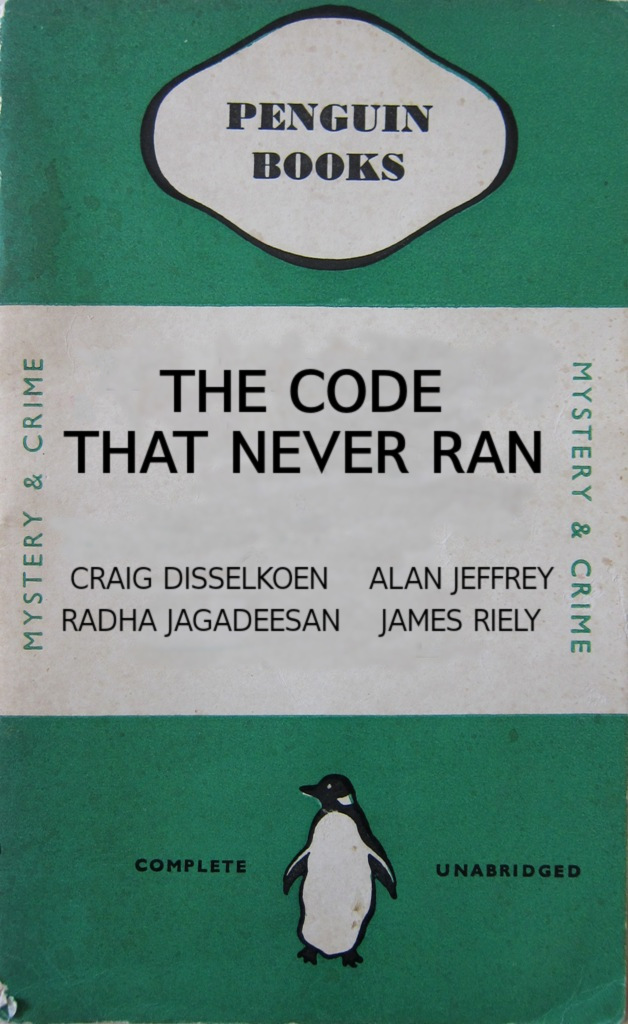
\includegraphics[height=.9\textheight]{green-penguin.jpg}
  \begin{minipage}[b][.9\textheight]{0.55\textwidth}\raggedleft
    A classic locked-room mystery.\\
    Eve was in the false branch\\
    of a conditional the whole time,\\
    \emph{how could she do it}?

    \vss

    \tiny
    
\includegraphics[height=1.5ex]{cc-by-88x31.png}~Creative Commons Attribution-ShareAlike 4.0

    Mozilla Research \textbar~DePaul University \textbar~U.~California San Diego
  \end{minipage}
\end{frame}

\section{Introduction}
\begin{frame}
  \frametitle{3 January 2018}

  \vskip.4\textheight
  
  {~~~\hskip.5\textwidth A day out at the Tate Modern}
  
  \vskip-.4\textheight
  
  {~\hskip.1\textwidth\rotatebox{5}{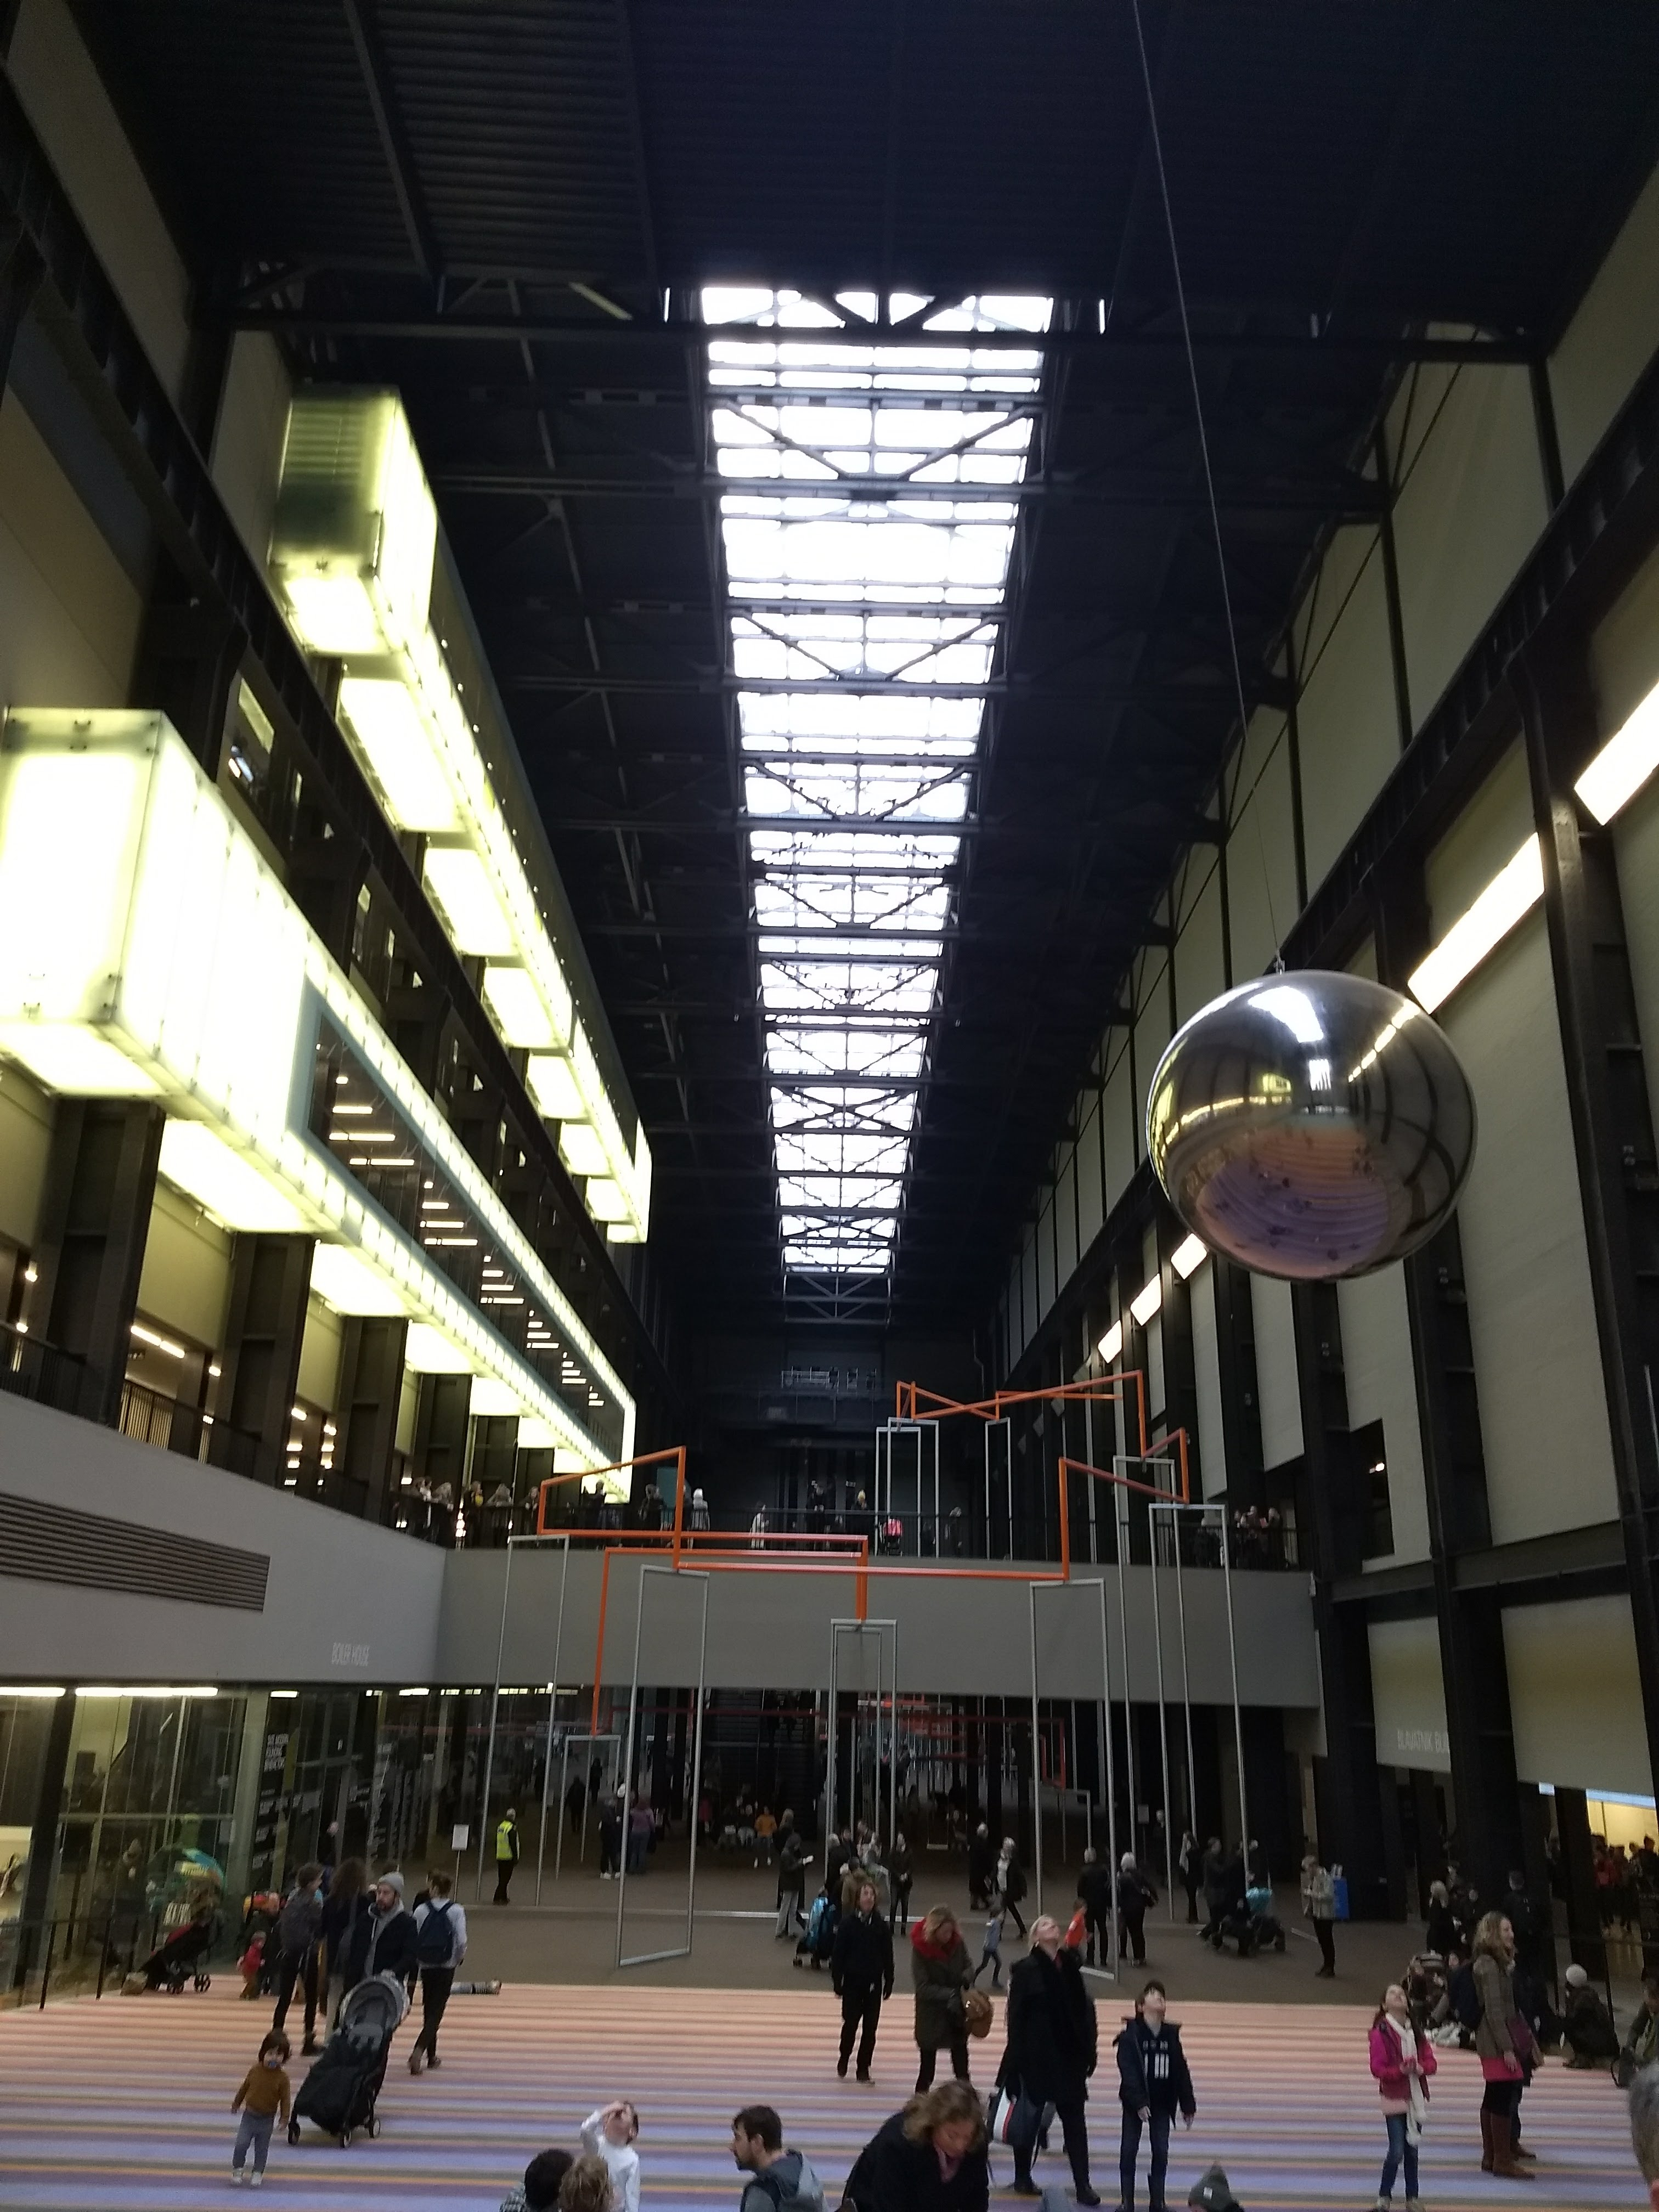
\includegraphics[height=.7\textheight]{turbine-hall-pendulum.jpg}}}

  \vskip-.7\textheight

  \onslide<2->{~\hskip.4\textwidth\rotatebox{-15}{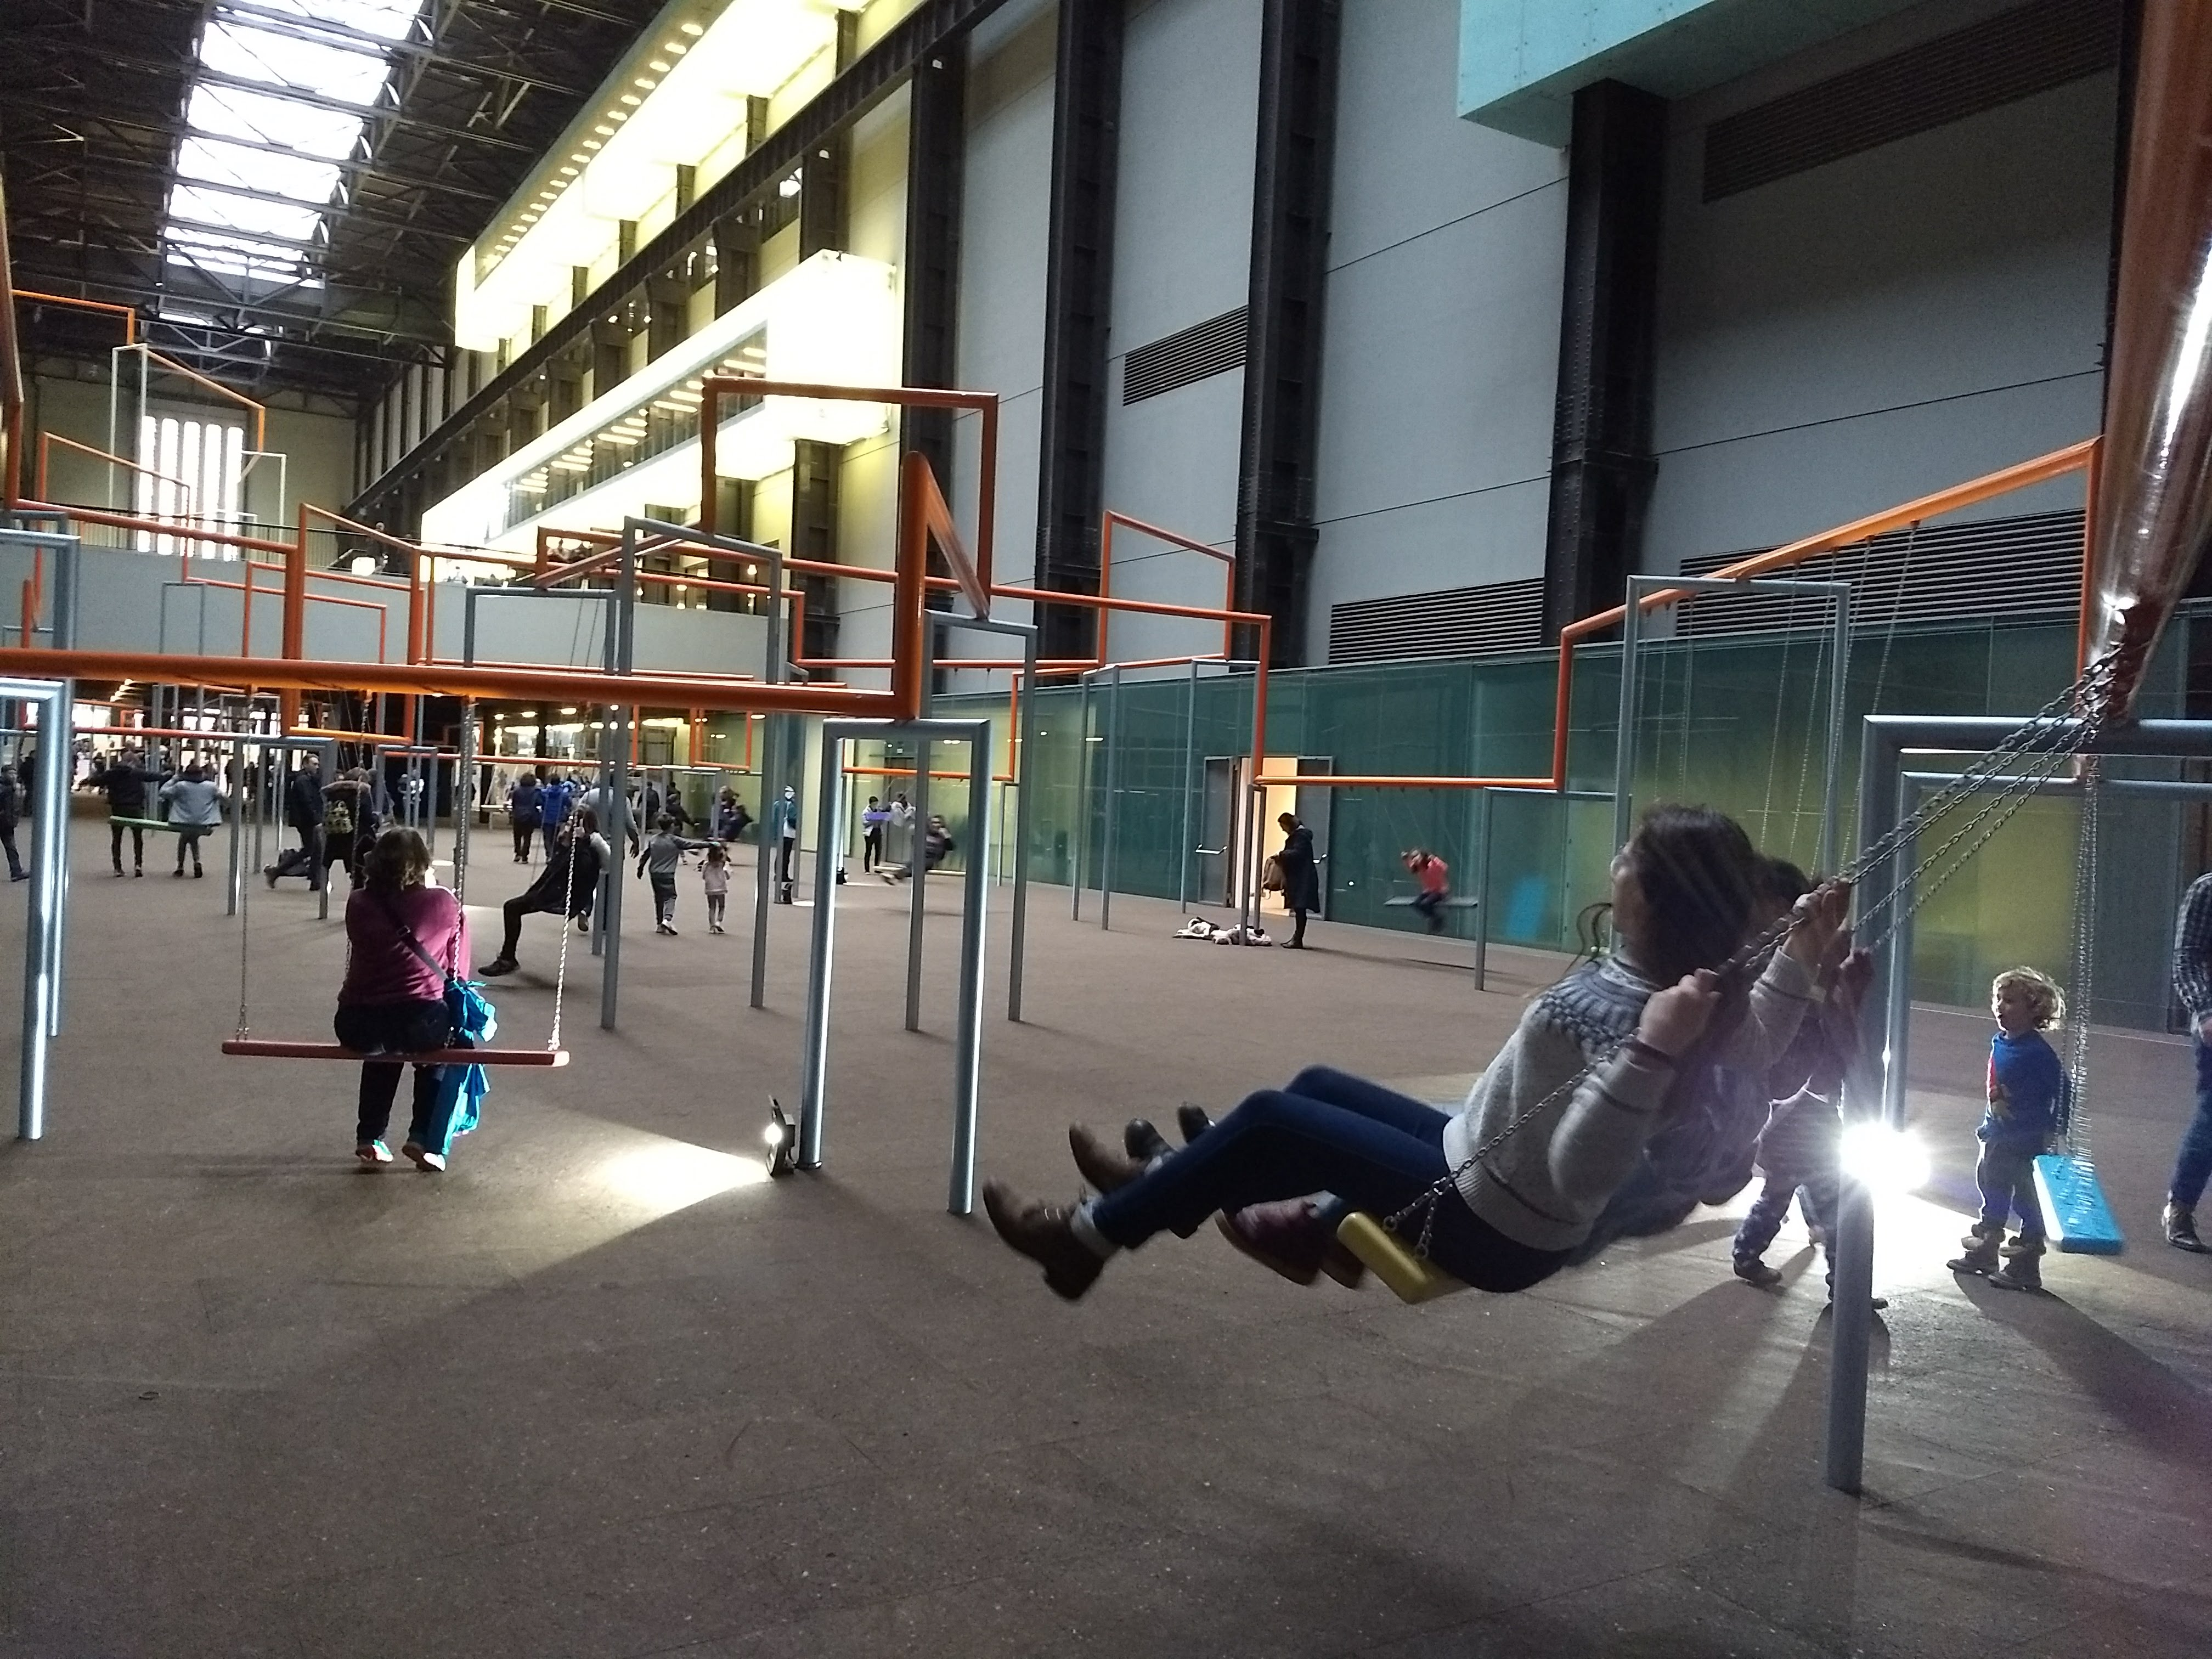
\includegraphics[height=.5\textheight]{turbine-hall-swings.jpg}}}

  \vskip-.8\textheight

  \onslide<3->{~\hskip.3\textwidth\fboxrule=1ex\fboxsep=0pt\fbox{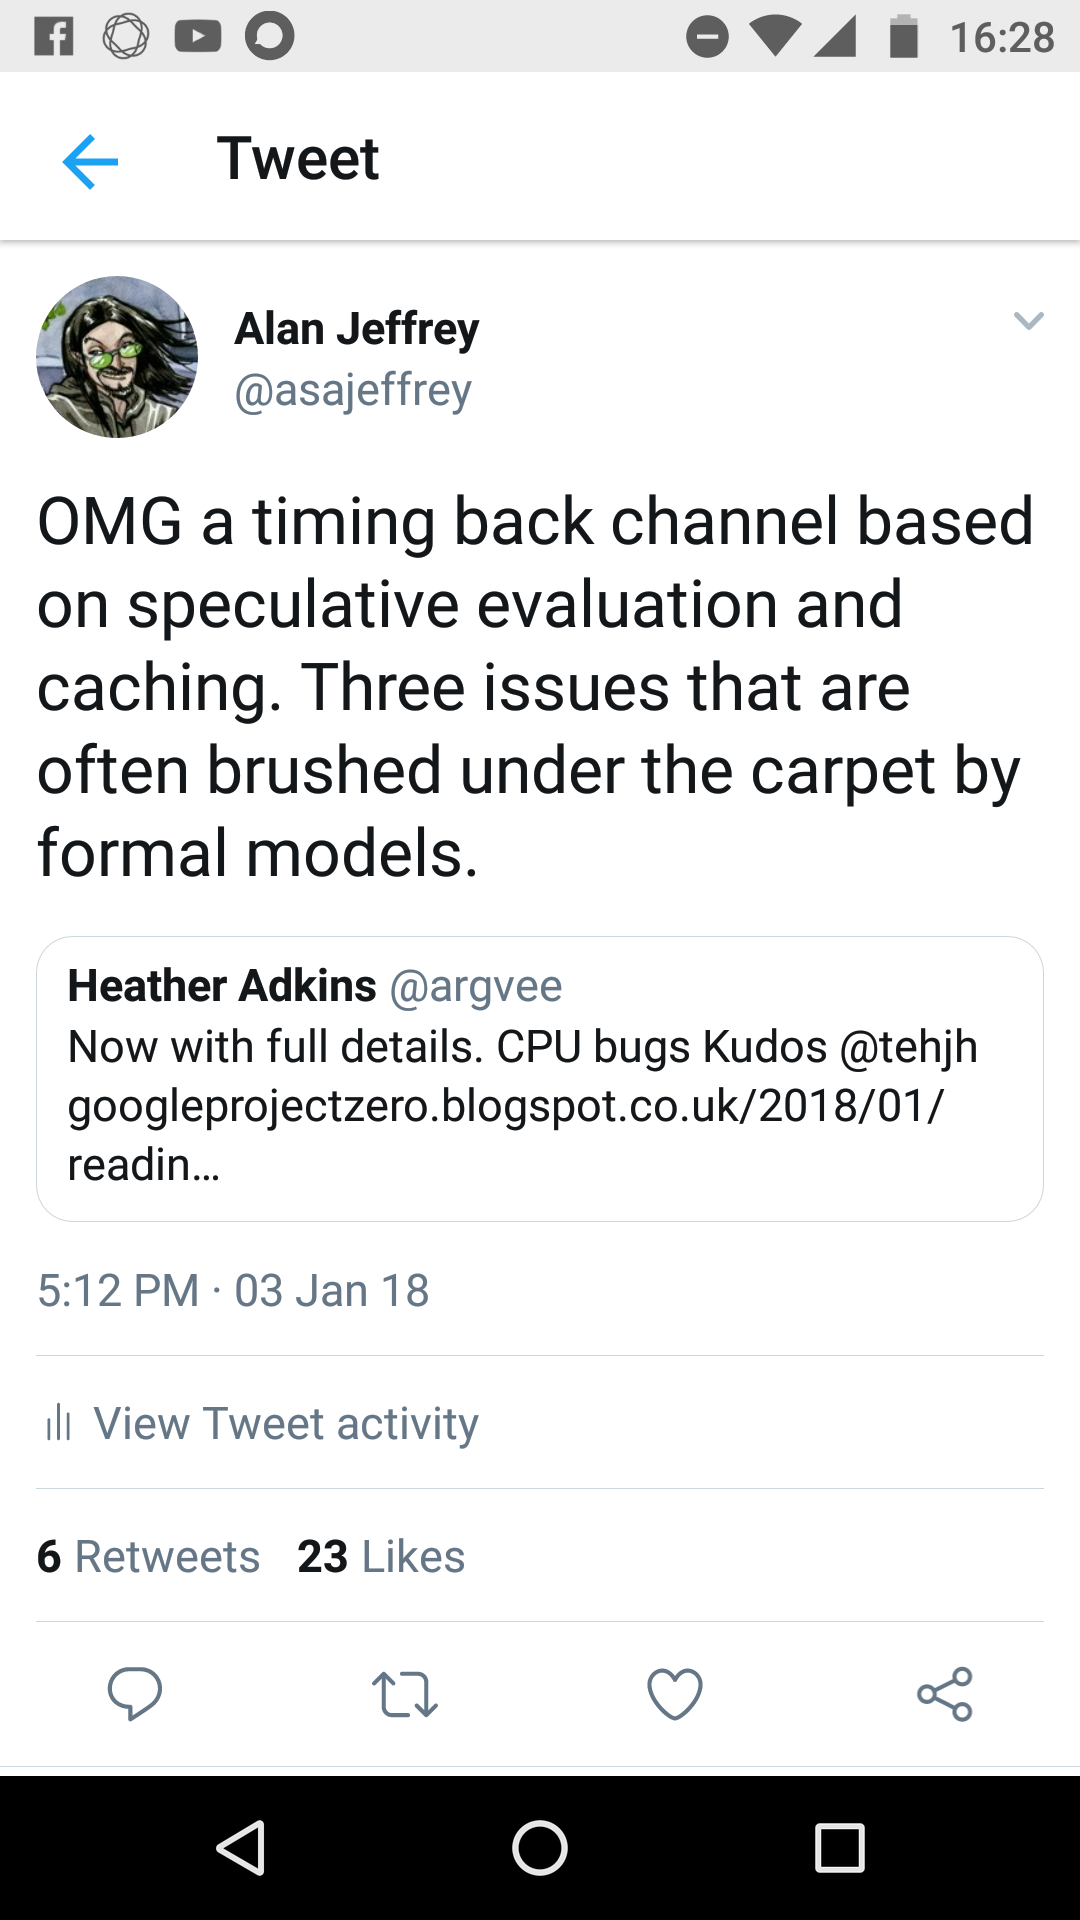
\includegraphics[height=.8\textheight]{omg-tweet.png}}}

\end{frame}

\section{Spectre}
\begin{frame}
  \frametitle{Spectre}

  {\fboxrule=1ex\fboxsep=0pt\fbox{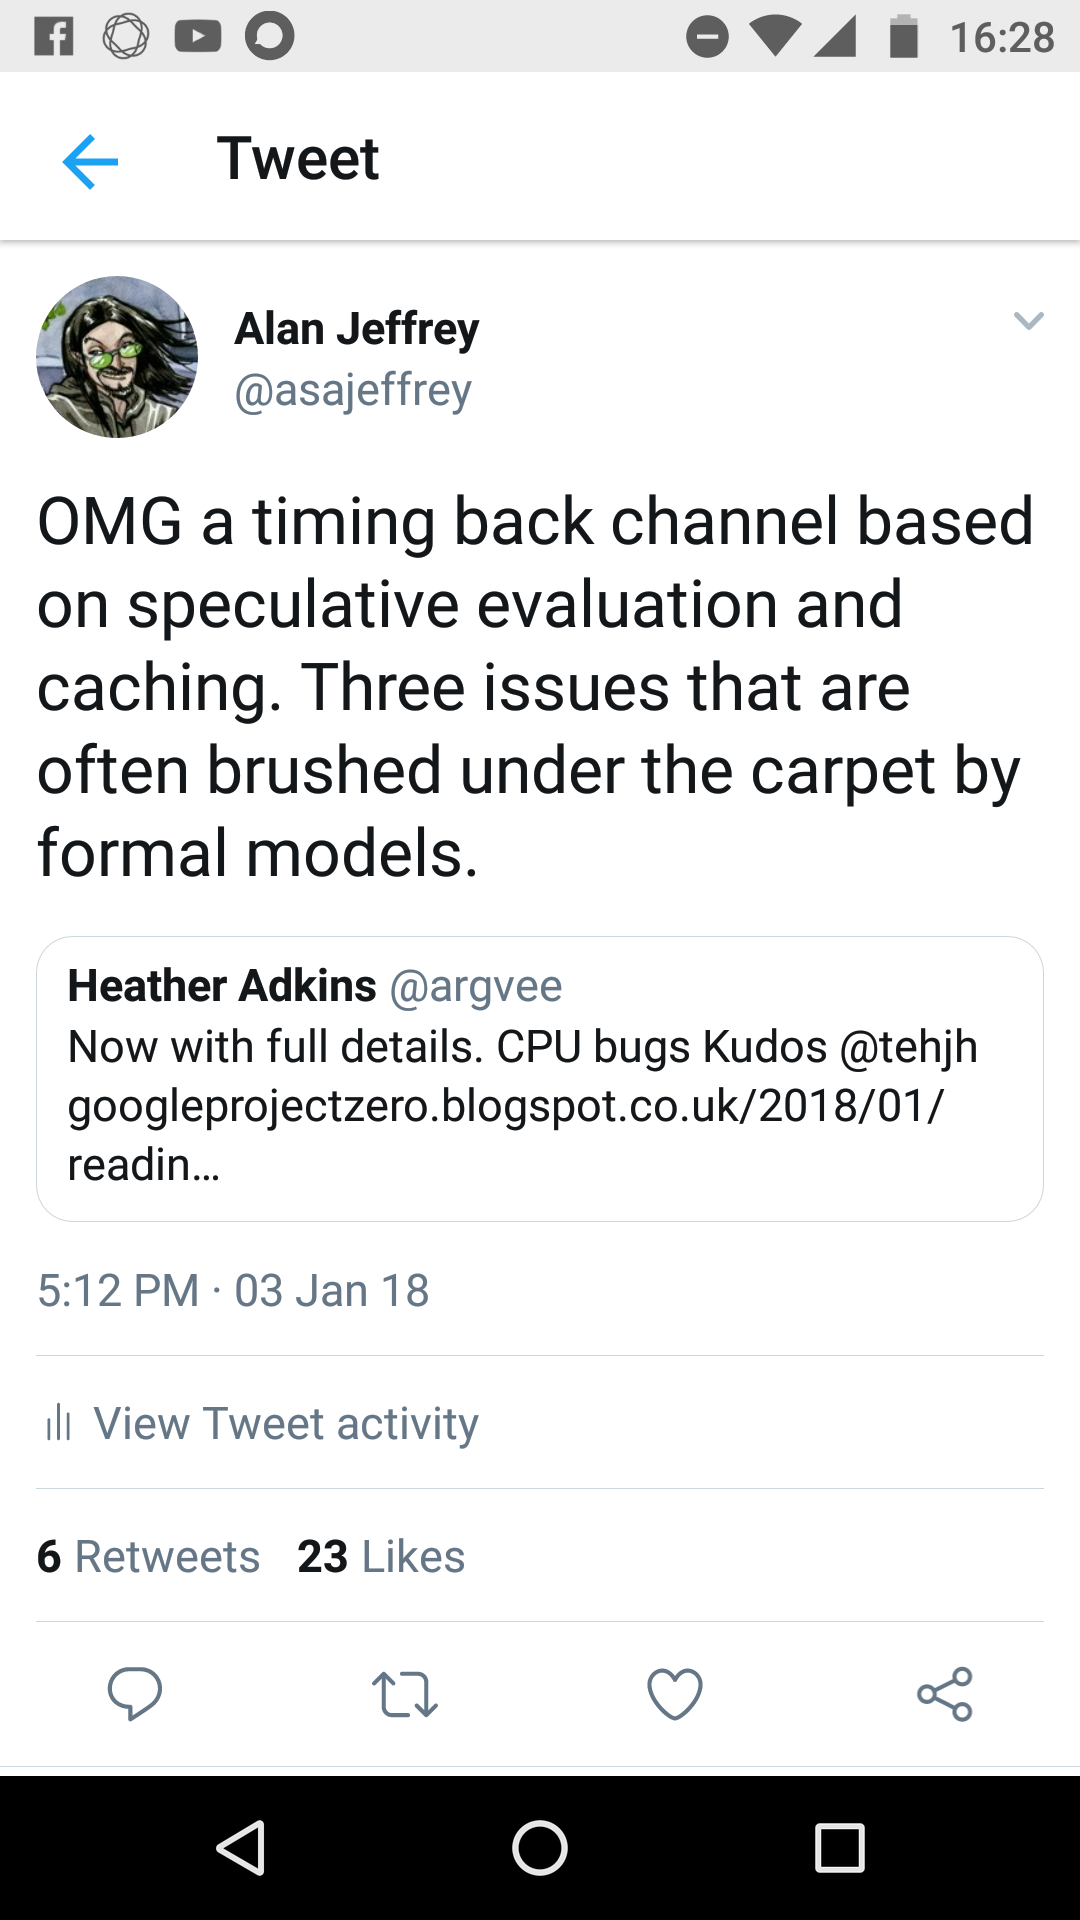
\includegraphics[height=.8\textheight]{omg-tweet.png}}}\quad
  \begin{minipage}[b]{.6\textwidth}\raggedright
    Attacks bypass run-time security checks.
    
    \bigskip
    Can bypass array bounds checks,\\
    and read whole process memory.

    \bigskip
    Can be exploited from JS,\\
    so evil.ad.com can read your bank.com data.

    \bigskip
    Attacks \emph{speculative evaluation}\\
    hardware optimization.
    
  \end{minipage}
\end{frame}

\section{Optimizations}
\begin{frame}
  \frametitle{Optimizations in hardware}
  
  A lie we tell programmers:\\
  ``computers execute instructions one after the other.''

  \[ \aLoc\GETS\aLoc+1\SEMI \bLoc\GETS1 \]

  has execution\only<2>{ where $\DW\bLoc1$ might happen first}:
  
\[\begin{tikzpicture}[node distance=1em]
  \event{rx1}{\DR{\aLoc}{1}}{}
  \event{wx2}{\DW{\aLoc}{2}}{right=of rx1}
  \event{wy1}{\DW{\bLoc}{1}}{right=of wx2}
  \po{rx1}{wx2}
  \only<1>{\po{wx2}{wy1}}
\end{tikzpicture}\]

  \pause

  \pause Shared-memory concurrency leaks the abstraction

  \medskip
  \pause Resulted in entire research area: weak memory models (e.g.~Pugh \emph{et al.}; C11)

\end{frame}

\begin{frame}
  \frametitle{Optimizations in hardware\onslide<4->{ and compilers}}

  Another lie we tell programmers:\\
  ``only one branch of an $\IF$ is executed.''

  \[ \IF(\aLoc)\THEN \bLoc\GETS1\SEMI\cLoc\GETS1 \ELSE \bLoc\GETS2\SEMI\cLoc\GETS1 \FI \]

  has execution%
  \only<2>{ where $\DW\cLoc1$ might happen before $\DW\bLoc1$}%
  \only<3>{ where $\DW\bLoc2$ might happen, then get rolled back}%
  \only<4>{ where $\DW\cLoc1$ might happen first}:
 
\[\begin{tikzpicture}[node distance=1em]
  \event{rx1}{\DR{\aLoc}{1}}{}
  \event{wy1}{\DW{\bLoc}{1}}{right=of rx1}
  \event{wz1}{\DW{\cLoc}{1}}{right=of wy1}
  \onslide<3->{\nonevent{nwy2}{\DW{\bLoc}{2}}{below=of wy1}}
  \onslide<3>{\nonevent{nwz1}{\DW{\cLoc}{1}}{right=of nwy2}}
  \po{rx1}{wy1}
  \onslide<1>{\po{wy1}{wz1}}
  \onslide<2-3>{\po[out=30,in=150]{rx1}{wz1}}
  \onslide<3->{\po{rx1}{nwy2}}
  \onslide<3>{\po{rx1}{nwz1}}
\end{tikzpicture}\]

  \pause\pause\pause\pause
  No language-level model for this!

  \medskip
  As weak memory models are to OOO, so \emph{what} is to speculation?

\end{frame}

\section{Simplified Spectre}
\begin{frame}
  \frametitle{Simplified Spectre}

  Imagine a $\SEC$, protected by a run-time security check:
  \[
     \IF \CANREAD(\SEC) \THEN \dots\mbox{use } \SEC\dots \ELSE \dots \FI
  \]
  For attacker code $\CANREAD(\SEC)$ is always false\pause, e.g.
\[\begin{tikzpicture}[node distance=1em]
  \event{ry1}{\DR{y}{1}}{}
  \event{wx2}{\DW{x}{2}}{right=of ry1}
  \nonevent{rs1}{\DR{\SEC}{1}}{below=of wx2}
  \nonevent{wx1}{\DW{x}{1}}{right=of rs1}
  \po{ry1}{wx2}
  \po{ry1}{rs1}
  \po{rs1}{wx1}
\end{tikzpicture}\]
  is an execution of
  \(
     \IF y \THEN \IF \CANREAD(\SEC) \THEN x\GETS\SEC \ELSE x\GETS2 \FI \FI
  \).

  \pause\bigskip
  Attacker goal: learn if $\SEC$ is $0$ or $1$.
  
\end{frame}

\begin{frame}
  \frametitle{Simplified Spectre}

  A very simplified Spectre attack:
  \[\begin{array}{l}
    \IF \CANREAD(\SEC) \THEN a[\SEC]\GETS1
    \brELIF \TOUCHED(a[0]) \THEN x\GETS0 
    \brELIF \TOUCHED(a[1]) \THEN x\GETS1 \FI 
  \end{array}\]
  with execution
\[\begin{tikzpicture}[node distance=1em]
  \nonevent{rs1}{\DR{\SEC}{1}}{}
  \nonevent{wa1}{\DW{a[1]}{1}}{right=of rs1}
  \cloud{ta1}{magic!} {right=of wa1}
  \event{wx1}{\DW{x}{1}} {right=of ta1}
  \po{rs1}{wa1}
  \po{wa1}{ta1}
  \po{ta1}{wx1}
\end{tikzpicture}\]
  Information flow from $\SEC$ to $x$,
  \emph{if} there's an implementation of ``magic''.

  \pause\bigskip
  \emph{Narrator}: there was one.
\end{frame}

\section{Results}
\begin{frame}
  \frametitle{Results}
  Formalization of pretty pictures
  as \emph{partially ordered multisets} (Gisher, 1988).

  \bigskip
  
  Compositional semantics 
  based on weak memory models (e.g.~C11).

  \bigskip

  Examples modeling Spectre, Spectre mitigations,\\
  PRIME+ABORT attack on transactional memory\dots\\
  \pause and a new family of attacks on compiler optimizations.
\end{frame}

\begin{frame}
  \frametitle{Modeling an attack on compiler optimizations}

  An attacker running two threads (initially $x=y=0$):
\[\begin{array}[t]{lcl}
  y\GETS x
  & \PAR
  & \begin{array}[t]{@{}l}
    \IF(y\EQ0)\THEN x\GETS1
    \brELIF(\CANREAD(\SEC))\THEN x\GETS\SEC
    \brELSE x\GETS1\SEMI z\GETS1 \FI
\end{array}\end{array}\]

If $\SEC$ is $1$, there is an execution:
\[\begin{tikzpicture}[node distance=1em]
  \event{rx1}{\DR{x}{1}}{}
  \event{wy1}{\DW{y}{1}}{below=of rx1}
  \event{ry1}{\DR{y}{1}}{right=5em of wy1}
  \event{wx1}{\DW{x}{1}}{above=of ry1}
  \event{wz1}{\DW{z}{1}}{right=of ry1}
  \po{rx1}{wy1}
  \po{ry1}{wz1}
  \rf{wx1}{rx1}
  \rf{wy1}{ry1}
\end{tikzpicture}\]

If $\SEC$ is $2$, there is no execution (due to cyclic dependency):
\[\begin{tikzpicture}[node distance=1em]
  \event{rx1}{\DR{x}{1}}{}
  \event{wy1}{\DW{y}{1}}{below=of rx1}
  \event{ry1}{\DR{y}{1}}{right=5em of wy1}
  \event{wx1}{\DW{x}{1}}{above=of ry1}
  \nonevent{wx2}{\DW{x}{2}}{right=of wx1}
  \event{wz1}{\DW{z}{1}}{right=of ry1}
  \po{rx1}{wy1}
  \po{ry1}{wx1}
  \po{ry1}{wx2}
  \po{ry1}{wz1}
  \rf{wx1}{rx1}
  \rf{wy1}{ry1}
\end{tikzpicture}\]

\end{frame}

\section{Experiments}
\begin{frame}
  \frametitle{Implementing attacks on compiler optimizations}

  Spectre and Prime+Abort are implemented.

  \bigskip
  Can we implement the attacks on compiler optimizations?

  \pause\bigskip
  \emph{Yes}\pause, under unrealistic assumptions:
  \begin{itemize}
  \item $\SEC$ is a constant known at compile-time
  \item $\CANREAD(\SEC)$ is a run-time check
  \end{itemize}

\end{frame}

\newcommand<>\highlightbox[2]{
  \alt#3{\makebox[\dimexpr\width-2\fboxsep]{\colorbox{#1}{#2}}}{#2}
}
\begin{frame}
  \frametitle{Implementing an attack on load/store reordering}

  Main attacker thread:
  \(
    x\GETS1\SEMI
    \IF (\CANREAD(\SEC)) \THEN x\GETS\SEC\SEMI \FI
    r\GETS y\SEMI
  \)

  \pause\medskip

{\footnotesize\fbox{\parbox[t]{.45\textwidth}{\raggedright When $\SEC \neq 1$, gcc generates:\\[\medskipamount]
{\color{bottle}\ttfamily
~~~~~~mov canReadSecret(\%rip), \%eax\\
~~~~~{\highlightbox<3->{bottle!80!black}{\color<3->{white}mov \$1, x(\%rip)}}\\
~~~~~~test \%eax, \%eax\\
~~~~~~je label1\\
~~~~~~mov \$0, x(\%rip)\\
~~~~label1:\\
~~~~~{\highlightbox<3->{orange!80!black}{\color<3->{white}mov y(\%rip), \%eax}}}\\[\medskipamount]
\onslide<3->{Writes $x$ then reads $y$}}}
\fbox{\parbox[t]{.45\textwidth}{\raggedright When $\SEC = 1$, gcc generates:\\[\medskipamount]
{\color{bottle}\ttfamily
~~~~~~mov canReadSecret(\%rip), \%eax\\
~~~~~{\highlightbox<4->{orange!80!black}{\color<4->{white}mov y(\%rip), \%eax}}\\
~~~~~{\highlightbox<4->{bottle!80!black}{\color<4->{white}mov \$1, x(\%rip)}}}\\~\\~\\~\\[\medskipamount]
\onslide<4->{Conditional has been eliminated!\\
Reads $y$ then writes $x$}}}}

\pause\pause\pause\bigskip
  Forwarding thread $x \GETS y$ allows attacker to spot the reordering

\end{frame}

\begin{frame}
  \frametitle{Implementing an attack on load/store reordering}

  Small delay between
  write $x$ and read $y$:
  increases probability of round trip

  \bigskip
  gcc will reorder across 30 straight-line instructions

  \bigskip
  Repeat to leak multiple bits, error correction

  \bigskip
  Bitwise accuracy 99.99\% at 300Kbps

\end{frame}

\begin{frame}
  \frametitle{Implementing an attack on dead store elimination}

  A similar attack targets dead store elimination

  \bigskip
  Works on clang + gcc

  \bigskip
  Bitwise accuracy 99.99\% at 1.2Mbps

\end{frame}

\section{Conclusions}
\begin{frame}
  \frametitle{Contributions}

  A compositional model of program execution that includes speculation.

  \bigskip
  Examples
  including existing information flow attacks on branch prediction\\
  and transactional memory, and new attacks on optimizing compilers.

  \bigskip
  Experimental evidence that the new attacks can be carried out,\\
  but only against compile-time secrets.

  \bigskip
  (Phew, we failed to mount attacks on JIT compilers.)

  \bigskip
  \bigskip
  \bigskip
  \bigskip
  \url{https://github.com/chicago-relaxed-memory/spec-eval}
\end{frame}


% \begin{frame}
%   \frametitle{Thank you!}
%   \url{https://github.com/chicago-relaxed-memory/spec-eval}
% \end{frame}

\end{document}

\section{Introduction}

\begin{frame}[fragile]
  \frametitle{Why? Spectre!}

  {\fboxrule=1ex\fboxsep=0pt\fbox{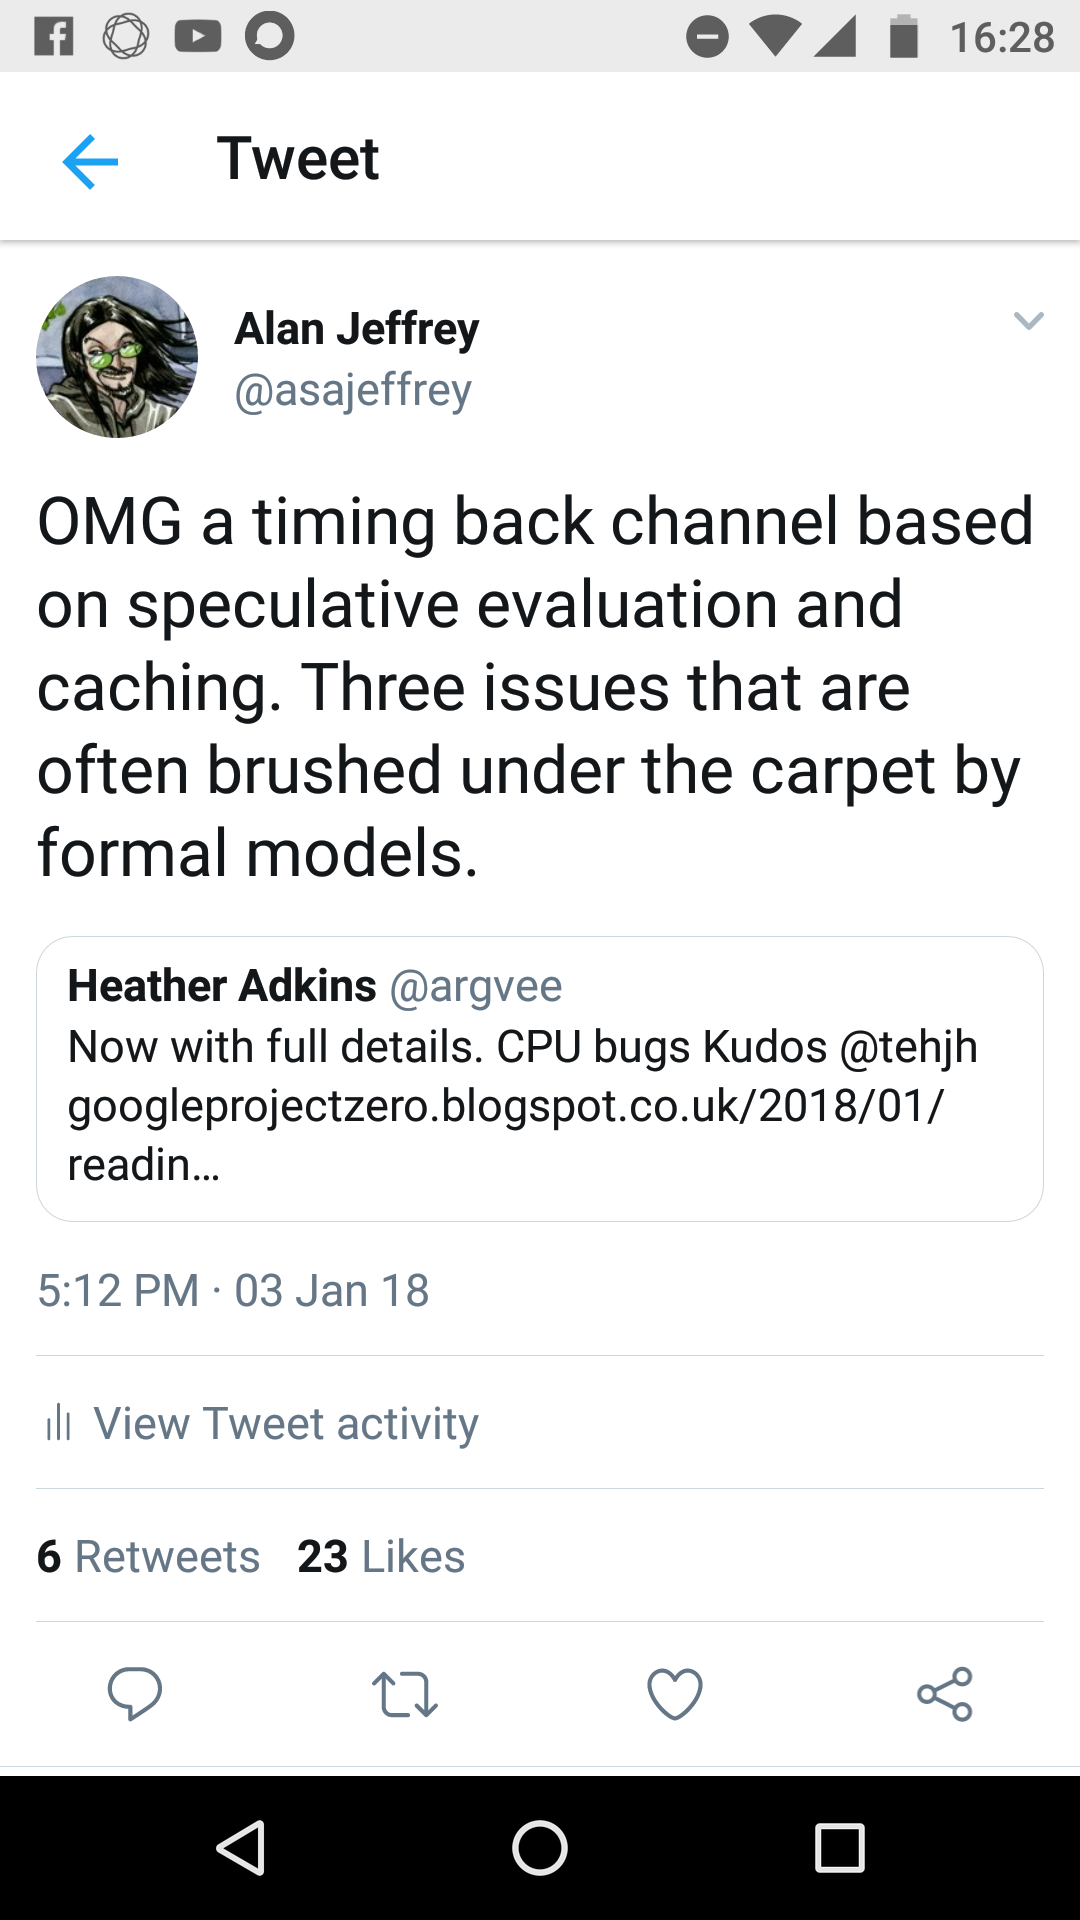
\includegraphics[height=.8\textheight]{omg-tweet.png}}}\quad\pause
  \begin{minipage}[b]{.45\textwidth}\raggedright
    Allows reding whole process address space.
    
    \bigskip
    Attacks bypass dynamic security checks:

\begin{verbatim}
if canRead(SECRET) {
  doStuffWith(SECRET);
}
\end{verbatim}
    Most formal models ignore code in branches
    that aren't taken.

    \bigskip
  \end{minipage}
\end{frame}

\begin{frame}
  \frametitle{Models that include speculation?}

  There are some models that include speculation\\
  \emph{relaxed memory models}:

  \begin{itemize}\footnotesize
  \item \emph{The Java Memory Model}\\
    Manson, Pugh and Adve, 2005.
  \item \emph{Generative Operational Semantics for Relaxed Memory Models}\\
    Jagadeesan, Pitcher and Riely, 2010.
  \item \emph{A promising semantics for relaxed-memory concurrency}\\
    Kang, Hur, Lahav, Vafeiadis and Dreyer, 2017.
  \end{itemize}

  \pause
  \emph{Question}: is there a simple model similar to
  those of relaxed memory, that can model speculation?
\end{frame}

\begin{frame}
  \frametitle{Information flow attacks on speculation}
  Speculation happens in many places:
  \begin{itemize}\footnotesize
  \item \emph{Speculation in hardware} (branch prediction,\ldots) \\
    \onslide<2->{Attacked by Spectre (Kocher \emph{et al.}~2019).}
  \item \emph{Transactions} (transactional memory,\ldots)\\
    \onslide<2->{Attacked by Prime+Abort (Disselkoen \emph{et al.}~2017).}
  \item \emph{Relaxed memory} (compiler optimizations,\ldots)\\
    \onslide<2->{No known attacks.}
  \end{itemize}
  
  \pause
  \emph{Question}: are there information flow attacks against
  compiler optimizations?
\end{frame}

\begin{frame}
  \frametitle{Contributions}
  \begin{itemize}\footnotesize
  \item A simple compositional model.
  \item Attacks (including a new attack on relaxed memory).
  \item Experiments (testing practicality of new attacks).
  \end{itemize}
\end{frame}

\section{Model}
\begin{frame}
  \frametitle{Pomsets}
  C11-style models are based on \emph{events} \\
  with \emph{labels} (e.g.~$(\DR{x}{3})$ or~$(\DW{x}{3})$)\\
  and \emph{relations} (e.g.~happens-before or reads-from).

  \bigskip\pause
  Simplest such is \emph{partially ordered multisets} (Gisher, 1988).

  \bigskip
  Only one relation, a partial order modeling dependency\pause, e.g.

\[\only<3>{\begin{tikzpicture}[node distance=1em]
  \event{rx1}{\DR{\aLoc}{1}}{}
  \event{wy1}{\DW{\bLoc}{1}}{right=of rx1}
  \event{wz2}{\DW{\cLoc}{2}}{right=of wy1}
  \po[out=25,in=155]{rx1}{wz2}
\end{tikzpicture}}
\only<4>{\begin{tikzpicture}[node distance=1em]
  \event{rx1}{\DR{\aLoc}{1}}{}
  \event{wy1}{\DW{\bLoc}{1}}{right=of rx1}
  \nonevent{wy2}{\DW{\bLoc}{2}}{below=of wy1}
  \po{rx1}{wy1}
  \po{rx1}{wy2}
\end{tikzpicture}}
\]

  \only<3>{is an execution of $(\aReg\GETS\aLoc\SEMI \bLoc\GETS1\SEMI \cLoc\GETS\aReg+1)$.}

  \only<4>{is an execution of $(\IF(\aLoc)\THEN \bLoc\GETS1 \ELSE \bLoc\GETS2 \FI)$.}
\end{frame}

\subsection{Loads and stores}
\begin{frame}
  \frametitle{Compositional pomset model}

  First off, straight-line code.

  \pause\bigskip
  \emph{New idea}: put preconditions on events\pause, e.g.

\[\begin{tikzpicture}[node distance=1em]
  \onslide<5->{\event{rx1}{\DR{\aLoc}{1}}{}}
  \onslide<4->{\event{wy1}{\DW{\bLoc}{1}}{right=of rx1}}
  \onslide<3->{\event{wz2}{\only<3-4>{r=1\mid}\only<5>{1=1\mid} \DW{\cLoc}{2}}{right=of wy1}}
  \onslide<5->{\po[out=25,in=155]{rx1}{wz2}}
\end{tikzpicture}\]

  is an execution of $(\onslide<5->{\aReg\GETS\aLoc\SEMI} \onslide<4->{\bLoc\GETS1\SEMI} \cLoc\GETS\aReg+1)$.

  \bigskip
  \only<4>{\emph{Note}: no dependency because $\aReg$ does not depend on $\bLoc\GETS1$.}

  \only<5>{\emph{Note}: dependency because $\aReg$ depends on $\aReg\GETS\aLoc$.}

  \only<5>{\emph{Also note}: performing a substitution $[1/\aReg]$.}

  \only<6>{\emph{Visualize}: elide tautologies}
\end{frame}

\subsection{Conditionals}
\begin{frame}
  \frametitle{Compositional pomset model}

  Next, conditionals.

  \pause\bigskip
  \emph{New idea}: an execution of $\IF M \THEN \aCmd \ELSE \bCmd \FI$\\
  comes from an execution of $\aCmd$ \emph{and} an execution of $\bCmd$\pause, e.g.

\[\begin{tikzpicture}[node distance=1em]
  \onslide<6->{\event{rx1}{\DR{\aLoc}{1}}{}}
  \onslide<3,5->{\event{wy1}{\only<3,5>{\aReg\neq0 \mid}\only<6>{1\neq0 \mid} \DW{\bLoc}{1}}{right=of rx1}}
  \onslide<4-6>{\event{wy2}{\only<4,5>{\aReg=0 \mid}\only<6->{1=0 \mid} \DW{\bLoc}{2}}{below=of wy1}}
  \onslide<7>{\nonevent{nwy2}{\DW{\bLoc}{2}}{below=of wy1}}
  \onslide<6->{\po{rx1}{wy1}}
  \onslide<6>{\po{rx1}{wy2}}
  \onslide<7>{\po{rx1}{nwy2}}
\end{tikzpicture}\]

  is an execution of \((
    \onslide<6->{\aReg\GETS\aLoc\SEMI}
    \onslide<5->{\IF(\aReg)\THEN}
    \onslide<3,5->{\bLoc\GETS1}
    \onslide<5->{\ELSE}
    \onslide<4->{\bLoc\GETS2}
    \onslide<5->{\FI}
  )\)
  \only<3>{when $\aReg\neq0$}
  \only<4>{when $\aReg=0$}

  \bigskip
  \only<7>{\emph{Visualize}: elide tautologies and cross out unsatisfiables}

\end{frame}


\begin{frame}
  \frametitle{Compositional pomset model}

  But\dots\pause
  any execution of $\aCmd$ should be\\
  an execution of $\IF M \THEN \aCmd \ELSE \aCmd \FI$\pause, e.g.

\[\begin{tikzpicture}[node distance=1em]
  \event{rx1}{\DR{\aLoc}{1}}{}
  \event{wy1}{\DW{\bLoc}{1}}{right=of rx1}
  \nonevent{nwy1}{\DW{\bLoc}{1}}{below=of wy1}
  \po{rx1}{wy1}
  \po{rx1}{nwy1}
\end{tikzpicture}\]
  is an execution of $(\IF \aLoc\THEN \bLoc\GETS1 \ELSE \bLoc\GETS1 \FI)$\pause,
  but so is
\[\begin{tikzpicture}[node distance=1em]
  \event{rx1}{\DR{\aLoc}{1}}{}
  \event{wy1}{\DW{\bLoc}{1}}{right=of rx1}
\end{tikzpicture}\]

  \pause
  \emph{New idea}: events from different branches can merge.

\end{frame}

\subsection{Concurrency}
\begin{frame}
  \frametitle{Compositional pomset model}

  Lastly, concurrency.

  \bigskip\pause
  \emph{Old idea}: match reads with matching
  writes (\`a la C11)\pause, e.g.

\[\begin{tikzpicture}[node distance=1em]
  \event{ry1}{\DR{y}{1}}{}
  \event{wx1}{\DW{x}{1}}{below=of ry1}
  \event{rx1}{\DR{x}{1}}{right=2.5em of ry1}
  \event{wy1}{\DW{y}{1}}{below=of rx1}
  \po{ry1}{wx1}
  \rf{wx1}{rx1}
  \rf{wy1}{ry1}
\end{tikzpicture}\]

  is an execution of
\((
  x\GETS y \PAR r\GETS x\SEMI y \GETS 1
)\).

\end{frame}

\begin{frame}
  \frametitle{Compositional pomset model}

  Glossed over some details:
  \begin{itemize}\footnotesize
  \item 3-valued pomsets for negative constraints $d \ltN e$,
  \item sanity conditions on reads-from,
  \item precise rules for dependency,
  \item variable declaration,
  \item $\cdots$
  \end{itemize}
  All in the paper!
  
\end{frame}

\section{Attacks}

\begin{frame}
  \frametitle{Information flow example}
  Imagine a $\SEC$, protected by a run-time security check:
  \[
     \IF \CANREAD(\SEC) \THEN \dots\mbox{use } \SEC\dots \ELSE \dots \FI
  \]
  For attacker code $\CANREAD(\SEC)$ is always false\pause, e.g.
\[\begin{tikzpicture}[node distance=1em]
  \event{ry1}{\DR{y}{1}}{}
  \event{wx2}{\DW{x}{2}}{right=of ry1}
  \nonevent{rs1}{\DR{\SEC}{1}}{below=of wx2}
  \nonevent{wx1}{\DW{x}{1}}{right=of rs1}
  \po{ry1}{wx2}
  \po{ry1}{rs1}
  \po{rs1}{wx1}
\end{tikzpicture}\]
  is an execution of
  \(
     \IF y \THEN \IF \CANREAD(\SEC) \THEN x\GETS\SEC \ELSE x\GETS2 \FI \FI
  \).

  \pause\bigskip
  Attacker goal: learn if $\SEC$ is $0$ or $1$.
  
\end{frame}

\subsection{Branch prediction}
\begin{frame}
  \frametitle{Modeling Spectre attack}

  Spectre uses cache timing to discover if a memory location
  has been touched.

  \pause\bigskip
  Glossing over a lot of details, this is
  \[
     \IF \TOUCHED(x) \THEN \cdots \ELSE \cdots \FI
  \]

  \pause
  Modeled with a new action $(\DT{x})$\pause, e.g.
\[\begin{tikzpicture}[node distance=1em]
  \event{tx}{\DT{x}}{}
  \event{wy1}{\DW{y}{1}}{right=of tx}
  \po{tx}{wy1}
\end{tikzpicture}\]
  is an execution of
  \(
     \IF \TOUCHED(x) \THEN y\GETS1 \FI
  \).

  \pause\bigskip
  Require that if there is an event labeled $(\DT{x})$
  then there must be an event labeled $(\DR{x}{v})$ or $(\DW{x}{v})$.
  
\end{frame}

\begin{frame}
  \frametitle{Modeling Spectre attack}

  A very simplified Spectre attack:
  \[\begin{array}{l}
    \IF \CANREAD(\SEC) \THEN a[\SEC]\GETS1
    \brELIF \TOUCHED(a[0]) \THEN x\GETS0 
    \brELIF \TOUCHED(a[1]) \THEN x\GETS1 \FI 
  \end{array}\]
  \pause
  e.g.~with execution
\[\begin{tikzpicture}[node distance=1em]
  \nonevent{rs1}{\DR{\SEC}{1}}{}
  \nonevent{wa1}{\DW{a[1]}{1}}{right=of rs1}
  \event{ta1}{\DT{a[1]}} {right=of wa1}
  \event{wx1}{\DW{x}{1}} {right=of ta1}
  \po{rs1}{wa1}
  \po{wa1}{ta1}
  \po{ta1}{wx1}
\end{tikzpicture}\]
  Information flow from $\SEC$ to $x$.
  
\end{frame}

\subsection{Transactions}
\begin{frame}
  \frametitle{Modeling Prime+Abort attack}

  Prime+Abort is an information flow attack on Intel's transactional memory.
  So first model transactions\pause, e.g.

\[\begin{tikzpicture}[node distance=1em]
  \event{b}{\DB}{}
  \event{rx1}{\DR{x}{1}}{right=of b}
  \event{wx2}{\DW{x}{2}}{right=of rx1}
  \event{c}{\DC}{right=of wx2}
  \po{b}{rx1}
  \po{rx1}{wx2}
  \po{wx2}{c}
\end{tikzpicture}\]
  and
\[\begin{tikzpicture}[node distance=1em]
  \event{b}{\DB}{}
  \nonevent{rx1}{\DR{x}{1}}{right=of b}
  \nonevent{wx2}{\DW{x}{2}}{right=of rx1}
  \nonevent{c}{\DC}{right=of wx2}
  \po{b}{rx1}
  \po{rx1}{wx2}
  \po{wx2}{c}
\end{tikzpicture}\]
are executions of \(\BEGIN\SEMI x\GETS x+1\SEMI \END\)\pause, but \emph{not}
\[\begin{tikzpicture}[node distance=1em]
  \event{b}{\DB}{}
  \event{rx1}{\DR{x}{1}}{right=of b}
  \nonevent{wx2}{\DW{x}{2}}{right=of rx1}
  \nonevent{c}{\DC}{right=of wx2}
  \po{b}{rx1}
  \po{rx1}{wx2}
  \po{wx2}{c}
\end{tikzpicture}\]

  
\end{frame}

\begin{frame}
  \frametitle{Modeling Prime+Abort attack}

  Transactions are fine, but not if we add a reason for an abort.

  \bigskip
  If the attacker knows an aborted transaction does so
  because of a read/write or write/write conflict, then in
  \[\begin{array}{l}
    \IF \CANREAD(\SEC) \THEN a[\SEC]\GETS1 \FI \PAR{}\\
    \BEGIN\SEMI a[1]\GETS2\SEMI \texttt{loop}\SEMI \END\SEMI x\GETS1
  \end{array}\]
  the transaction aborts only when $\SEC$ is $1$.

  \[\begin{tikzpicture}[node distance=1em]
  \nonevent{rs1}{\DR{\SEC}{1}}{}
  \nonevent{wa1}{\DW{a[1]}{1}}{right=of rs1}
  \event{b}{\DB}{below=of rs1}
  \nonevent{wa2}{\DW{a[1]}{2}}{right=of b}
  \nonevent{c}{\DC}{right=of wa2}
  \event{wx1}{\DW{x}{1}}{right=of c}
  \po{rs1}{wa1}
  \po{b}{wa2}
  \po{wa2}{c}
  \po{c}{wx1}
  \rf{wa1}{wa2}
\end{tikzpicture}\]
  Information flow from $\SEC$ to $x$.

\end{frame}

\subsection{Compiler optimizations}
\begin{frame}
  \frametitle{New store reordering attack}

  An attack on relaxed memory,
  \emph{discovered from this model}.
\[\begin{array}[t]{@{}l}
    y\GETS x
  \PAR\begin{array}[t]{@{}l}
    \IF(y\EQ0)\THEN x\GETS1
    \brELIF(\CANREAD(\SEC))\THEN x\GETS\SEC
    \brELSE x\GETS1\SEMI z\GETS1 \FI
\end{array}\end{array}\]

If $\SEC$ is $1$, there is an execution:
\[\begin{tikzpicture}[node distance=1em]
  \event{rx1}{\DR{x}{1}}{}
  \event{wy1}{\DW{y}{1}}{below=of rx1}
  \event{ry1}{\DR{y}{1}}{right=2.5em of wy1}
  \event{wx1}{\DW{x}{1}}{above=of ry1}
  \event{wz1}{\DW{z}{1}}{right=of ry1}
  \po{rx1}{wy1}
  \po{ry1}{wz1}
  \rf{wx1}{rx1}
  \rf{wy1}{ry1}
\end{tikzpicture}\]

If $\SEC$ is $2$, there is no execution:
\[\begin{tikzpicture}[node distance=1em]
  \event{rx1}{\DR{x}{1}}{}
  \event{wy1}{\DW{y}{1}}{below=of rx1}
  \event{ry1}{\DR{y}{1}}{right=2.5em of wy1}
  \event{wx1}{\DW{x}{1}}{above=of ry1}
  \nonevent{wx2}{\DW{x}{2}}{right=of wx1}
  \event{wz1}{\DW{z}{1}}{right=of ry1}
  \po{rx1}{wy1}
  \po{ry1}{wx1}
  \po{ry1}{wx2}
  \po{ry1}{wz1}
  \rf{wx1}{rx1}
  \rf{wy1}{ry1}
\end{tikzpicture}\]

\end{frame}

\begin{frame}
  \frametitle{New dead store elimination attack}

\end{frame}

\begin{frame}
  \frametitle{New dead store elimination attack}

  Another attack
  \emph{discovered from this model}.
\[\begin{array}[t]{@{}l}
    y\GETS x
  \PAR\begin{array}[t]{@{}l}
    x\GETS 1\SEMI\\
    \IF(\CANREAD(\SEC))\THEN \IF(\SEC)\THEN x\GETS 2\FI
    \brELSE x\GETS 2\FI
\end{array}\end{array}\]
If $\SEC$ is $1$, there is an execution:
\[\begin{tikzpicture}[node distance=1em]
  \event{rx1}{\DR{x}{1}}{}
  \event{wy1}{\DW{y}{1}}{right=of rx1}
  \event{wx1}{\DW{x}{1}}{right=2.5em of wy1}
  \event{wx2}{\DW{x}{2}}{right=of wx1}
  \rf[out=160,in=20]{wx1}{rx1}
  \po{rx1}{wy1}
  \po{wx1}{wx2}
\end{tikzpicture}\]
\pause
If dead store elimination is performed, there is \emph{no} execution:
\[\begin{tikzpicture}[node distance=1em]
  \event{rx1}{\DR{x}{1}}{}
  \event{wy1}{\DW{y}{1}}{right=of rx1}
  \nonevent{nwx1}{\DW{x}{1}}{right=2.5em of wy1}
  \event{wx2}{\DW{x}{2}}{right=of wx1}
  \rf[out=160,in=20]{wx1}{rx1}
  \po{rx1}{wy1}
  \po{nwx1}{wx2}
\end{tikzpicture}\]

\end{frame}

\section{Experiments}
\begin{frame}
  \frametitle{Implementing the new attacks}

  Spectre and Prime+Abort are implemented.\\
  What about the attacks on compiler optimizations?

  \pause\bigskip
  \emph{Yes}\pause, under unrealistic assumptions:
  \begin{itemize}
  \item $\SEC$ is a constant known at compile-time,
  \item $\CANREAD(\SEC)$ is a run-time check.
  \end{itemize}

\end{frame}

\begin{frame}
  \frametitle{Implementing load/store reordering}

  x86 assembly generated by gcc for the main thread of a variant of the load-store reordering attack:
  \bigskip
  
\fbox{\parbox[t]{.45\textwidth}{\raggedright If $\SEC$ is $0$:\\\begin{alltt}\footnotesize
~~mov SECRET(\%rip), \%eax\\
~~mov \$1, x(\%rip)\\
~~test \%eax, \%eax\\
~~je label1\\
~~mov \$0, x(\%rip)\\
label1:\\
~~mov y(\%rip), \%eax\\
~~test \%eax, \%eax\\
~~sete \%eax
\end{alltt}Writes $x$ then reads $y$,\\so can read 1}}
\fbox{\parbox[t]{.45\textwidth}{\raggedright If $\SEC$ is $1$:\\\begin{alltt}\footnotesize
~~mov SECRET(\%rip), \%eax\\
~~mov y(\%rip), \%eax\\
~~mov \$1, x(\%rip)\\
~~test \%eax, \%eax\\
~~sete \%eax
\end{alltt}Reads $y$ then writes $x$,\\so cannot read 1}}

\bigskip
  A forwarding thread copies $x$ to $y$.

\end{frame}

\begin{frame}
  \frametitle{Implementing load/store reordering}

  To make this attack more likely, introduce\\
  a small delay between write of $x$ and read of $y$,\\
  increases probability of round trip.

  \bigskip
  Experimentally gcc will reorder load/store
  across 30 straight-line instructions.

  \bigskip
  Repeat attack to leak multiple bits,\\
  and increase probability of success.
  
  \bigskip
  Attack is 99.9\% accurate at 100Kbps.

\end{frame}

\begin{frame}
  \frametitle{Implementing dead store elimination attack}

  DSE attack is similar.

  \bigskip
  Works against clang as well as gcc.

  \bigskip
  Attack is 99.9\% accurate at 400Kbps (clang), 2Mbps (gcc).

\end{frame}

\section{Conclusions}
\begin{frame}
  \frametitle{Also in the paper}
  Details of the model, semantics, etc.

  \bigskip
  Temporal logic for proving invariants (e.g.~no thin-air read).

  \bigskip
  More examples.
\end{frame}
  
\begin{frame}
  \frametitle{Contributions}

  A model of program execution that includes speculation.

  \bigskip
  Examples
  including existing information flow attacks on
  branch prediction and transactional memory, and new attacks on optimizing compilers.

  \bigskip
  Experimental evidence about how practical it is to mount
  the new class of attacks.

  \bigskip
  A temporal logic which supports compositional proof.

  \bigskip\footnotesize
  \url{https://github.com/chicago-relaxed-memory/spec-eval}

\end{frame}

\end{document}
